%!TEX TS-program=xelatex
%!USE flag=shell-escape
\documentclass{beamer}
\usepackage{HSE-theme/beamerthemeHSE} % Подгружаем тему

%%% Работа с русским языком и шрифтами
\usepackage[english,russian]{babel}   % загружает пакет многоязыковой вёрстки
\usepackage{fontspec}      % подготавливает загрузку шрифтов Open Type, True Type и др.
\defaultfontfeatures{Ligatures={TeX},Renderer=Basic}  % свойства шрифтов по умолчанию
\setmainfont[Ligatures={TeX,Historic}]{Myriad Pro} %  установите шрифты Myriad Pro или (при невозможности) замените здесь на другой шрифт, который есть в системе — например, Arial
\setsansfont{Times New Roman}  %  установите шрифты Myriad Pro или (при невозможности) замените здесь на другой шрифт, который есть в системе — например, Arial
\setmonofont{Courier New}
\uselanguage{russian}
\languagepath{russian}
\deftranslation[to=russian]{Theorem}{Теорема}
\deftranslation[to=russian]{Definition}{Определение}
\deftranslation[to=russian]{Definitions}{Определения}
\deftranslation[to=russian]{Corollary}{Следствие}
\deftranslation[to=russian]{Fact}{Факт}
\deftranslation[to=russian]{Example}{Пример}
\deftranslation[to=russian]{Examples}{Примеры}

\usepackage{multicol}       % Несколько колонок
\graphicspath{{images/}}    % Папка с картинками


\usepackage{listings}

% графики всякие
\usepackage{qtree}
\usepackage{pgfplots}
    \pgfplotsset{
        compat=1.12,
    }
\usepackage{hyperref}

% \usepackage[backend=biber]{biblatex}
% \addbibresource{used_sources.bib}
\usepackage{caption}
\captionsetup{labelformat=simple}
\newlength{\mylen}


%%% Информация об авторе и выступлении
\title[Заголовок]{\footnotesize Факультет Компьютерных Наук\\Департамент
Программной Инженерии\\Выпускная квалификационная работа}
\subtitle{Криптографические алгоритмы и протоколы для распределенных реестров\\
Cryptographic Algorithms and Protocols for Distributed Ledgers}
\author[Куприянов К.И.]{\scriptsize Выполнил: студент
гр.БПИ151 Куприянов Кирилл\\Научный руководитель: Профессор, руководитель ДПИ,\\к.т.н. Авдошин Сергей Михайлович}
\institute[Высшая школа экономики]{}
\date{\the\year}

\begin{document}    % Начало презентации
\frame[plain]{
    \maketitle
}

% \frame[plain]{\titlepage} % Титульный слайд

% \section{Просто слайд с текстом}
% \subsection{Просто слайд с текстом}

\begin{frame}
\frametitle{Популярность блокчейна}
    \begin{figure}
        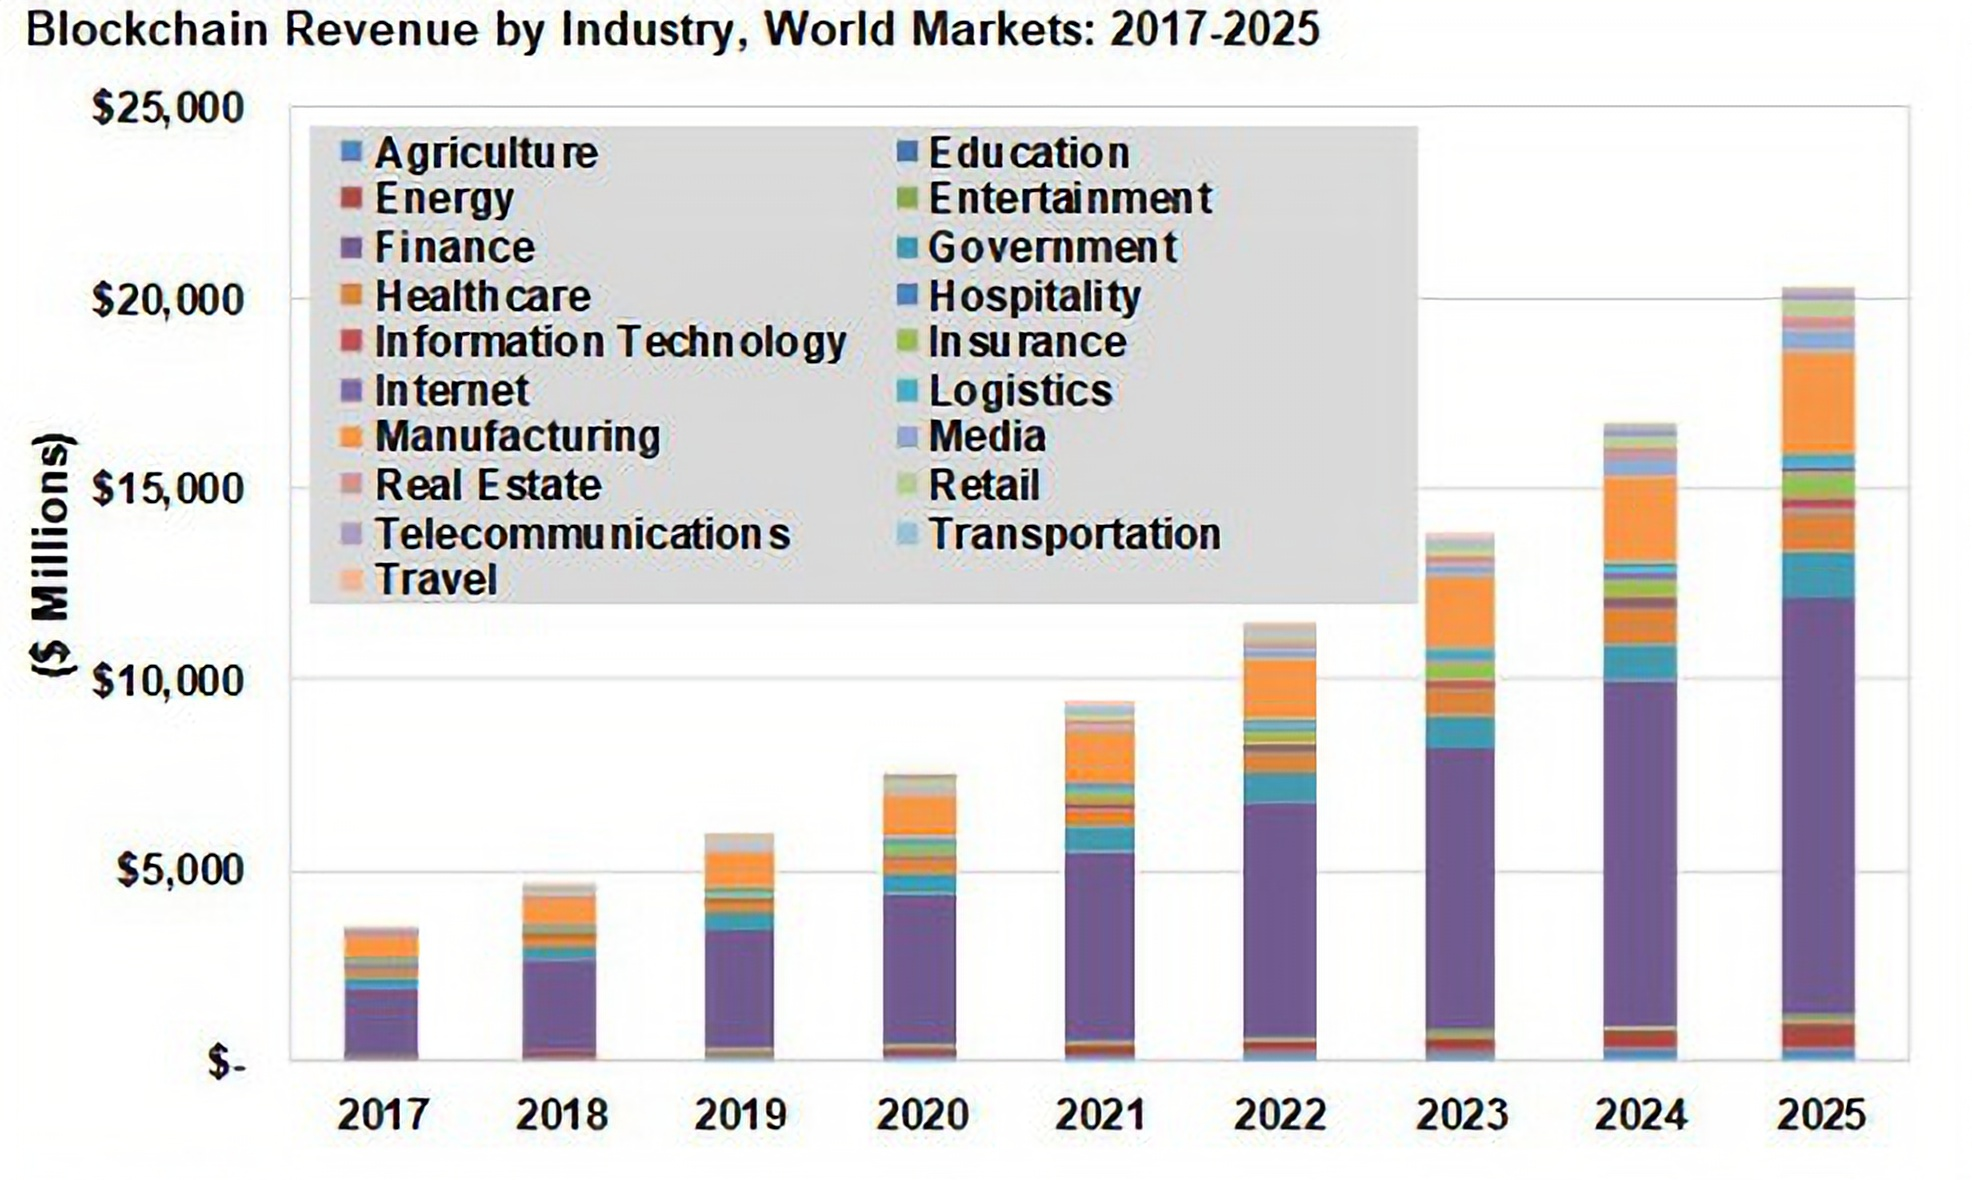
\includegraphics[width=0.85\textwidth]{graph}
        \caption{\small Рост выручки в индустриях с применением блокчейна [22]}
        %% CITE Niranjanamurthy, M., Nithya, B.N. & Jagannatha, S. Cluster Comput (2018). https://doi.org/10.1007/s10586-018-2387-5
    \end{figure}
    % \begin{multicols}{2}
    %     1. Распределённые реестры -- ``база данных'', которая распределена между
    %     несколькими сетевыми узлами или вычислительными устройствами. Каждый
    %     узел получает данные из других узлов и хранит полную копию реестра.
    %     Обновления узлов происходят независимо друг от друга

    %     \columnbreak

    %     2. Криптография -- наука, изучающая математические методы защиты
    %     информации, методы преобразования, обеспечивающие ее конфиденциальность
    %     и аутентичность.\\
    %     \emph{Разделы: асимметричные криптосистемы, системы электронной цифровой
    %     подписи (ЭЦП), хеш-функции}
    %     \medskip
    %     % \includegraphics[width=\columnwidth]{skidka.png}
    % \end{multicols}
\end{frame}

\begin{frame}
    \begin{figure}
        
\includegraphics[height=0.9\textheight]{tim_obl}
        \caption{Swanson, T., Great Chain of Numbers}
    \end{figure}
\end{frame}

% \setbeamercolor{background canvas}{bg=HSEgreen}
% \begin{frame}
%     \begin{multicols}{2}
%      ll   hekaj
%         \columnbreak
%     \end{multicols}
% \end{frame}
% \setbeamercolor{background canvas}{bg=white}

\begin{frame}
\frametitle{Определения}
\begin{itemize}
\small
    \item \emph{Распределённый реестр (Distributed Ledger)} --- распределённая база
          данных между сетевыми узлами. Каждый из узлов может получать данные
          других, при этом храня полную копию реестра.  Обновления этих
          узлов происходят независимо друг от друга
    \item \emph{Блокчейн} --- постоянно растущий список записей, называемых блоками,
          которые связаны и защищены с помощью криптографии. Он копируется его
          пользователями и устойчив к модификации
    \item \emph{Приватный и публичный ключи} --- сущности системы асимметричного
          шифрования для безопасной передачи сообщений между парой субъектов
    \item \emph{Цифровая подпись} --- реквизит электронного документа, полученный в
          результате криптографического преобразования информации и позволяющий
          проверить отсутствие искажения информации, принадлежность
          подписи владельцу сертификата ключа подписи
    \item \emph{Майнер} --- лицо, обеспечивающее достижение консенсуса о том,
          какие транзакции считать валидными с целью предотвращения траты уже
          использованной в другой транзакции монеты
\end{itemize}
\end{frame}

\begin{frame}[c]
    \small
    \frametitle{Цель и задачи}
    Расширить существующую классификацию по использованию в реестрах
    [30] алгоритмов и протоколов, а также создать приложение для
    автоматизации создания кода распределённого реестра.\\

    {\bfseries \color{HSEblue} Задачи}:
    \begin{itemize}
        \item Выявить популярные распределённые реестры; выделить и изучить
              криптографические алгоритмы и протоколы в ниммх
        \item Расположить их на диаграмме Эйлера-Венна для создания обновлённой
              классификации
        \item Реализовать код блокчейна с интерфейсом встраивания вариаций
              алгоритмов
        \item Создать модуль на языке Python3.6.5, позволяющий пользователю
              сгенерировать код работающего с использованием выбранных
              алгоритмов блокчейна
        \item Автоматизировать работу системы с набором существующих алгоритмов
    \end{itemize}
\end{frame}

\begin{frame}
    \frametitle{План}
    \begin{itemize}
        \item Вступление
        \item Источники информации
        \item Результат обновления классификации
        \item Описание программного решения
        \item Схема работы
        \item Особенности архитектуры
        \item Технологии реализации
        \item Заключение
    \end{itemize}
\end{frame}

\begin{frame}
    % \centering
    \begin{figure}
    
\includegraphics[width=3cm]{rg_logo}\pause
    \vfill
    
\includegraphics[width=6cm]{decentr_logo}\pause
    
\includegraphics[width=3cm]{wiki_logo}\pause
    
\includegraphics[width=3cm]{btcwiki_logo}\pause
    \hfill
    
\includegraphics[width=2cm]{reddit_logo}\pause
    
\includegraphics[width=2cm]{springer_logo}
        \caption{Источники информации ([1-2], [36], [39], [6], [22])}
    \end{figure}
\end{frame}

\begin{frame}
    \frametitle{Классификация от Tim Swanson [30]}
    \begin{figure}
        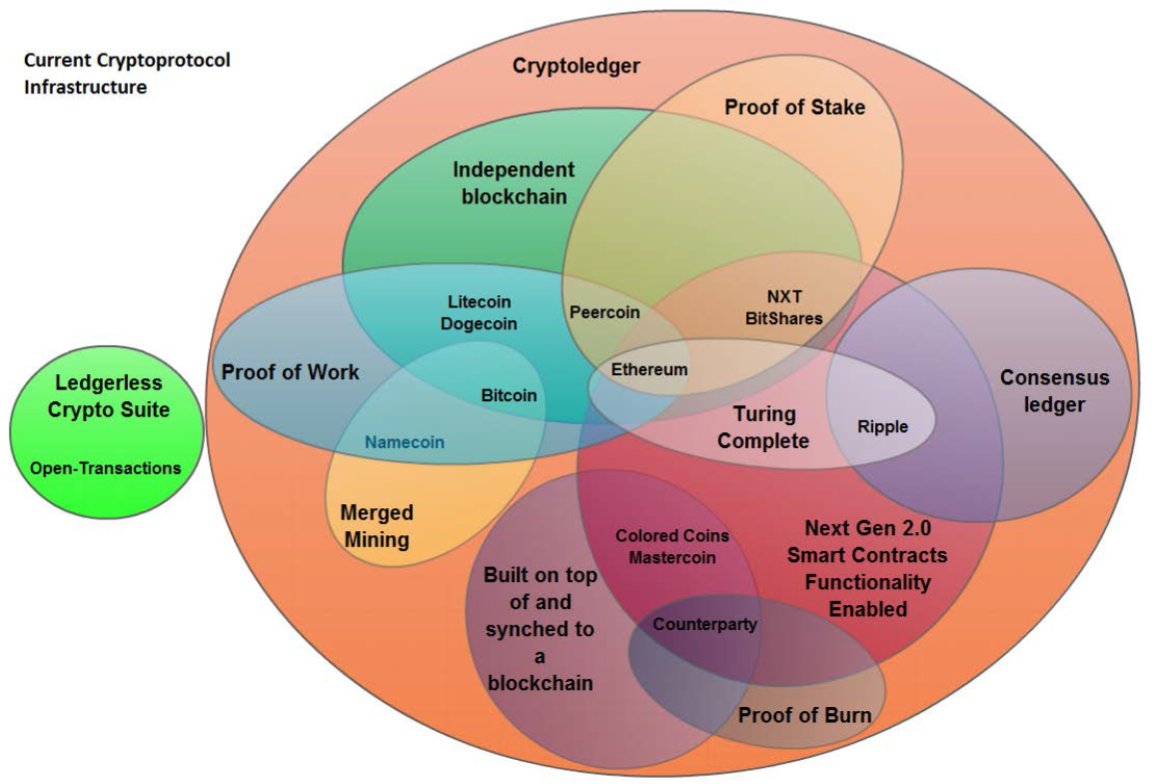
\includegraphics[width=0.9\columnwidth]{current_protocols}
        \caption{Криптопротокол по состоянию на 2014 год [30]}
    \end{figure}
\end{frame}

\begin{frame}
    \frametitle{Обновлённая классификция}
    \begin{figure}
        \centering
        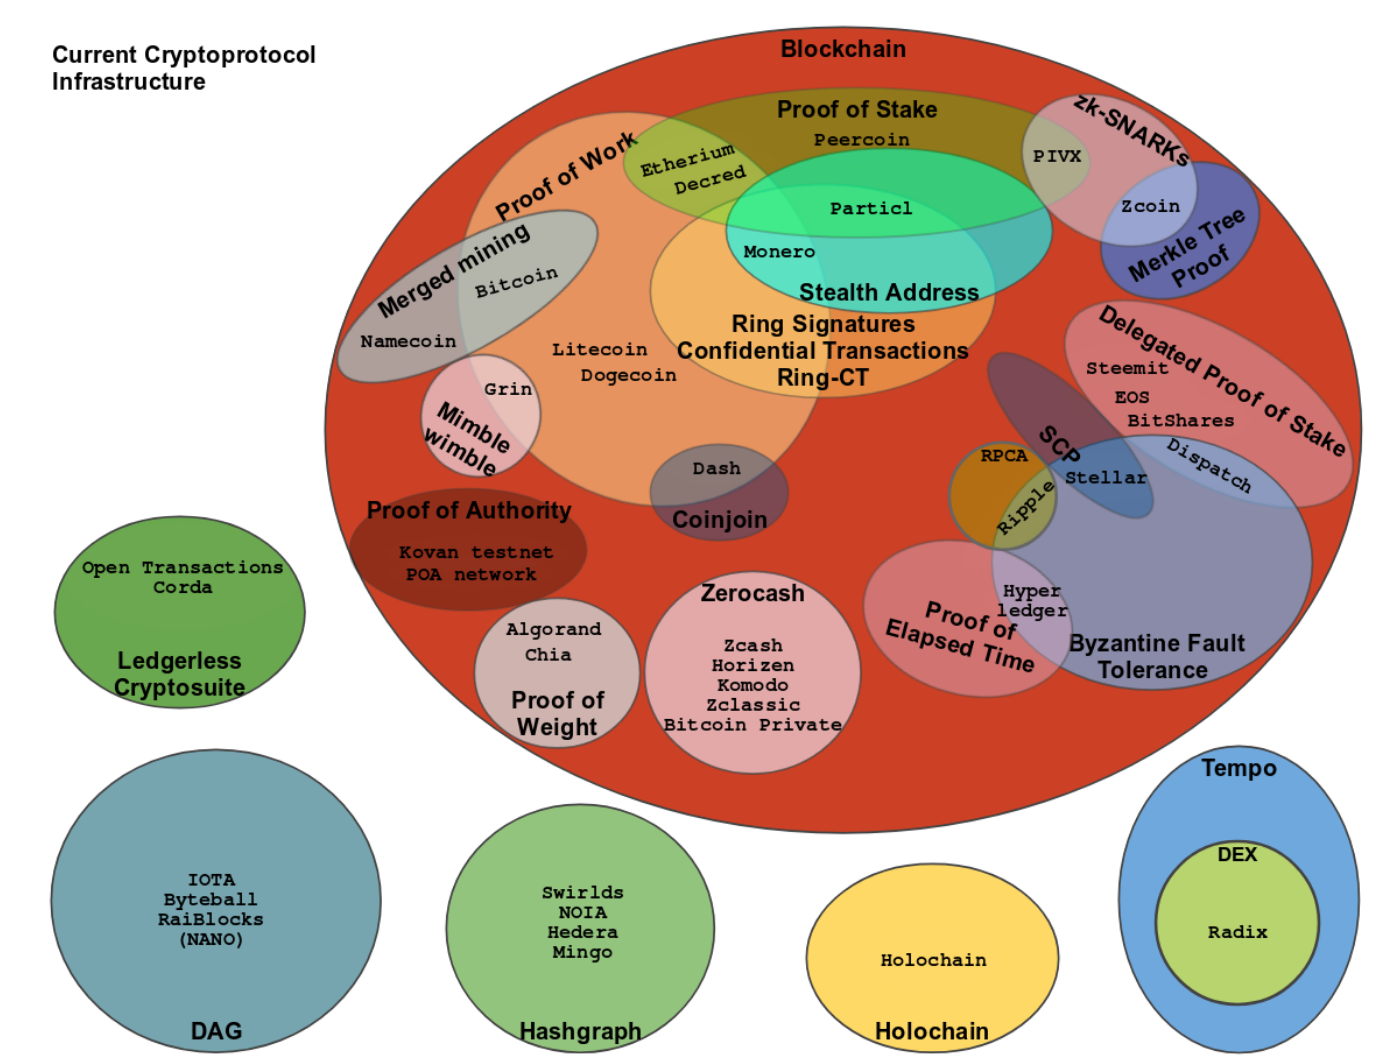
\includegraphics[width=0.8\columnwidth]{myprotocol_w_title}
        \caption{Криптопротокол по состоянию на 2019 год}
    \end{figure}
\end{frame}

\begin{frame}
    \frametitle{Аналоги предлагаемого программного решения}
    \begin{figure}
        \centering
        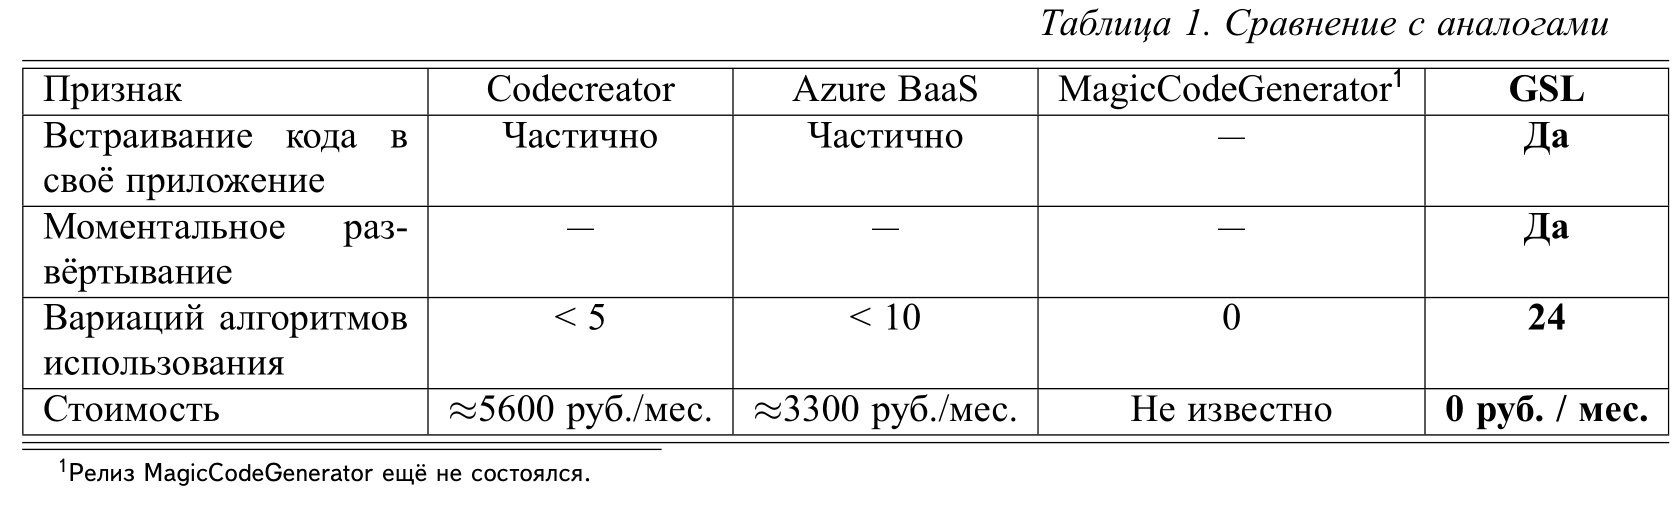
\includegraphics[width=\columnwidth]{analogues}
        
\includegraphics[width=0.6\columnwidth]{analogues_logos}
        \caption{\scriptsize Аналоги программного решения. Codecreator [7] и Azure BaaS [20]}
    \end{figure}
\end{frame}

\begin{frame}[c]
    \frametitle{Программа}
    \Large
    \begin{center}
    \begin{enumerate}
        \item Компоновщик
        \item Реализация блокчейна
    \end{enumerate}
    \end{center}
\end{frame}

\begin{frame}
    \frametitle{Схема работы компоновщика}
    \begin{figure}
        \centering
        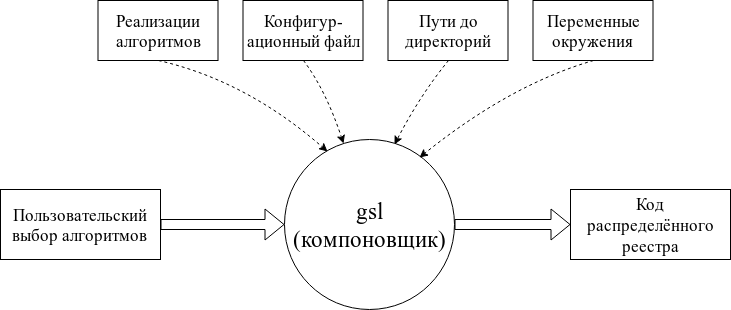
\includegraphics[width=0.9\textwidth]{komponovshik}
        \caption{\small Схема работы компоновщика}
    \end{figure}
\end{frame}

\begin{frame}
    \frametitle{Схема работы компоновщика}
    \vspace{0.6cm}
    \begin{figure}
        \centering
        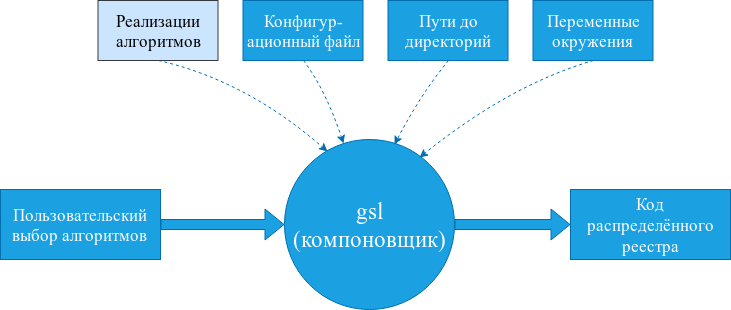
\includegraphics[width=0.9\textwidth]{komponovshik_color}
        \caption{\small \centering Схема работы компоновщика (с указанием
        степени принадлежности реализаций: синий --- собственная, голубой ---
        готовая)}
    \end{figure}
\end{frame}

\begin{frame}
    \frametitle{Программа}
    \begin{figure}
        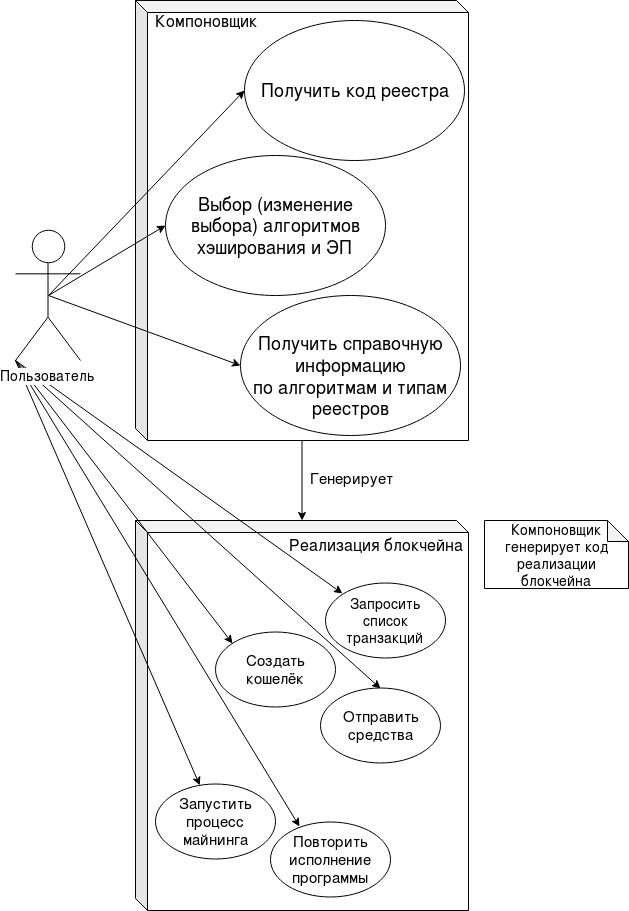
\includegraphics[height=0.75\textheight]{uc}
        \caption{Диаграмма use case}
    \end{figure}
\end{frame}

\begin{frame}
    \frametitle{Особенности архитектуры}
    \begin{itemize}
        % \item Не устанавливает лишних алгоритмов, а только то что выбрал
        %       \textbf{пользователь}
         \item \textbf{Сервер автообновления} поддерживает консистентность
              реализаций алгоритмов
         \item \textbf{Continuous integration} позволяет отслеживать
              работоспособность автообновляемой версии реализаций алгоритмов
        \item Спроектировано для упрощения дальнейшей \textbf{масштабируемости}
        \item Реализации алгоритмов были адаптированы под
              \textbf{Python3}
        \item Использование \textbf{конфигурационных} файлов вместо разрастания
              количества аргументов командной строки
    \end{itemize}
\end{frame}

\begin{frame}
    \frametitle{Сервер автообновления}
    \begin{figure}
        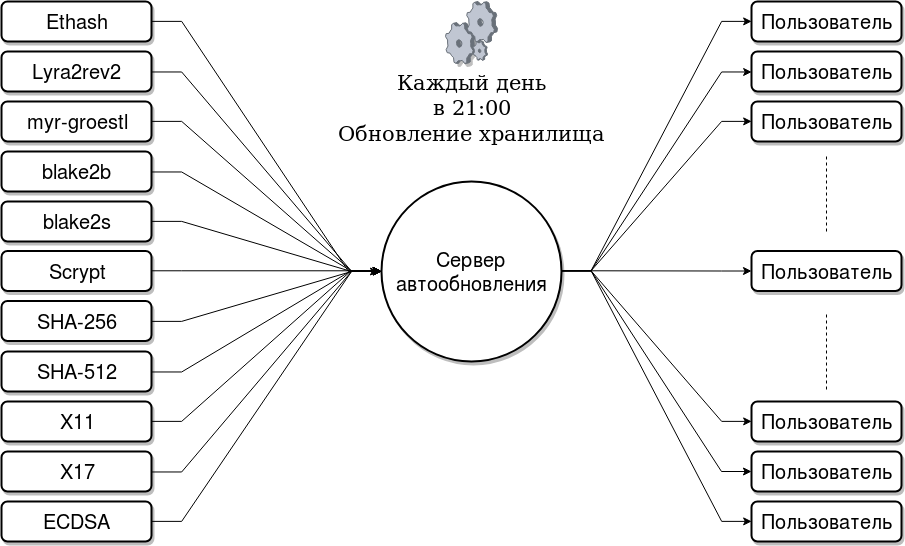
\includegraphics[width=\columnwidth]{server}
        \caption{\small Процесс работы автообновления}
    \end{figure}
\end{frame}

\begin{frame}
    \frametitle{Сервер автообновления}
    \begin{figure}
        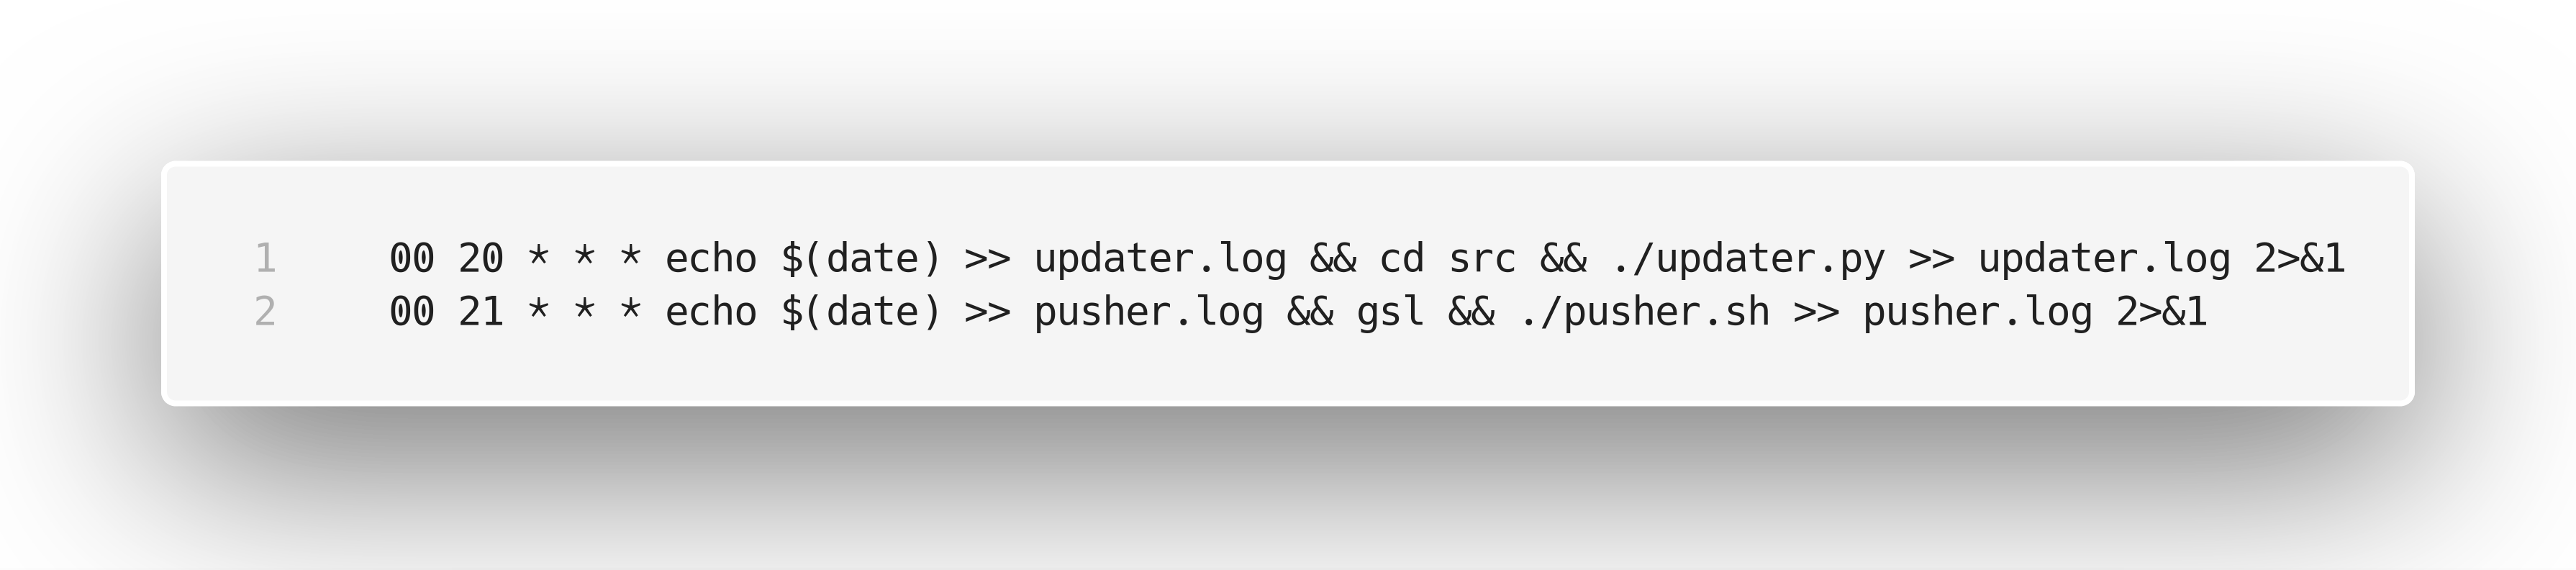
\includegraphics[width=\columnwidth]{cron}
        \caption{\small Регулярное (ежедневное) обновление}
    \end{figure}
\end{frame}

\begin{frame}
    \frametitle{Технологии реализации}
    \begin{figure}
        
\includegraphics[width=\columnwidth]{tech.png}
        \caption{\small Инструменты реализации}
    \end{figure}
\end{frame}

\setbeamercolor{background canvas}{bg=HSEblue}
\begin{frame}
    \centering
    \LARGE \bfseries \color{white}
    Демонстрация
\end{frame}
\setbeamercolor{background canvas}{bg=white}

\begin{frame}
    \frametitle{Выводы}
    \begin{itemize}
        \item[\checkmark] Устаревшая классификация обновлена
        \item[\checkmark] В новой отражены не только новые алгоритмы и
                          протоколы, но и современные распределённые реестры
        \item[\checkmark] Разработано средство автоматизации программирования
        \item[\checkmark] Создан автоматизированный процесс по работе с кодами
                          реализаций алгоритмов и их обновлению
    \end{itemize}
\end{frame}

\begin{frame}
    \frametitle{Направления дальнейшей работы}
    \begin{itemize}
        \item Новые реестры
        \item Новые алгоритмы
        \item Реализации алгоритмов Python $\rightarrow$ С
        \item Исследование новых реестров
        \item Поддержание актуальности классификации
    \end{itemize}
\end{frame}

\begin{frame}
    \frametitle{Список используемых источников}
    \begin{figure}
        \centering
        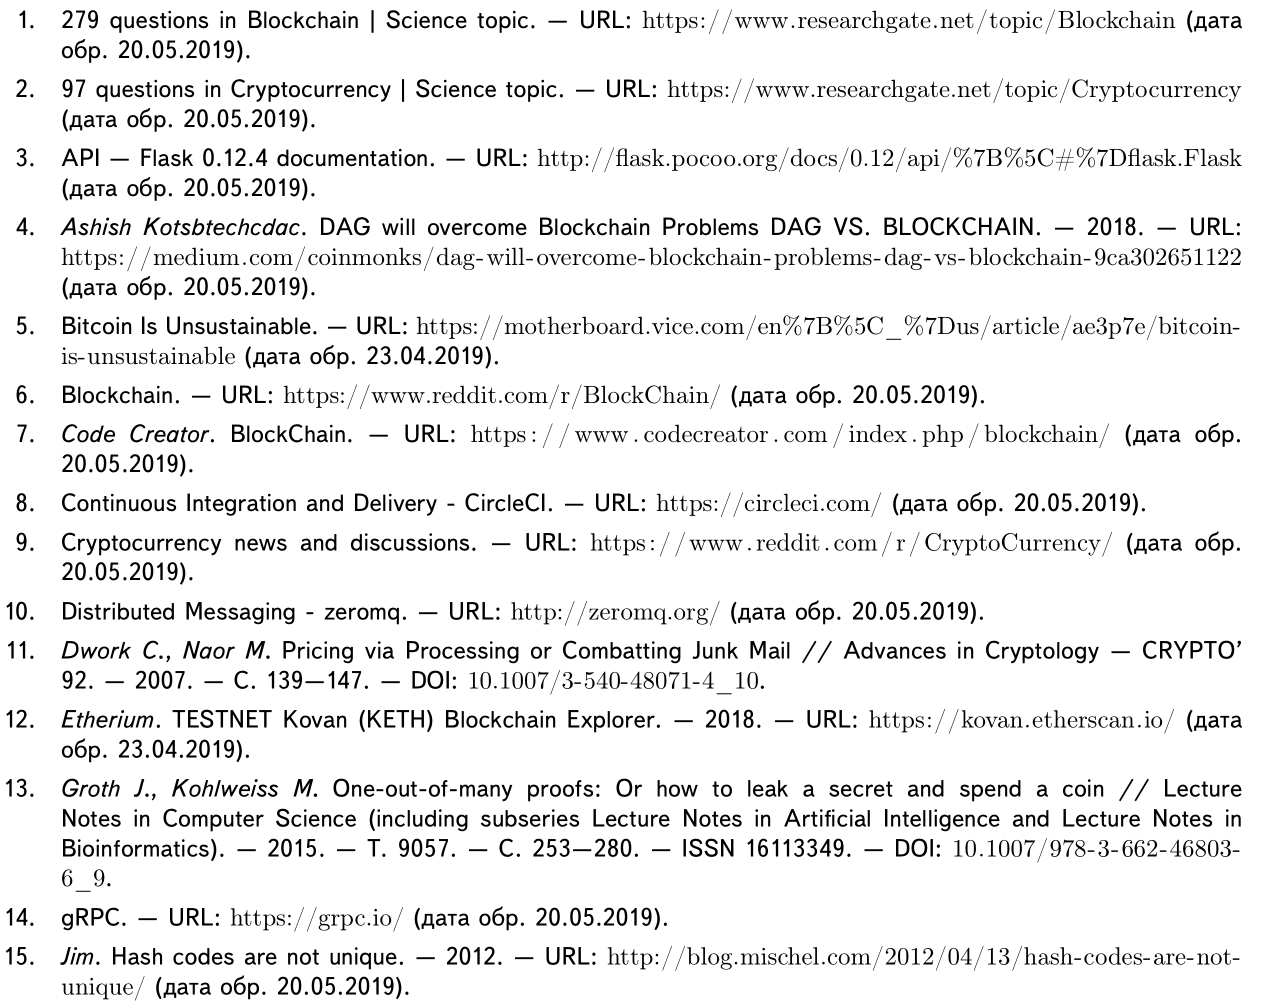
\includegraphics[width=0.85\textwidth]{lib1}
    \end{figure}
\end{frame}

\begin{frame}
    \frametitle{Список используемых источников}
    \begin{figure}
        \centering
        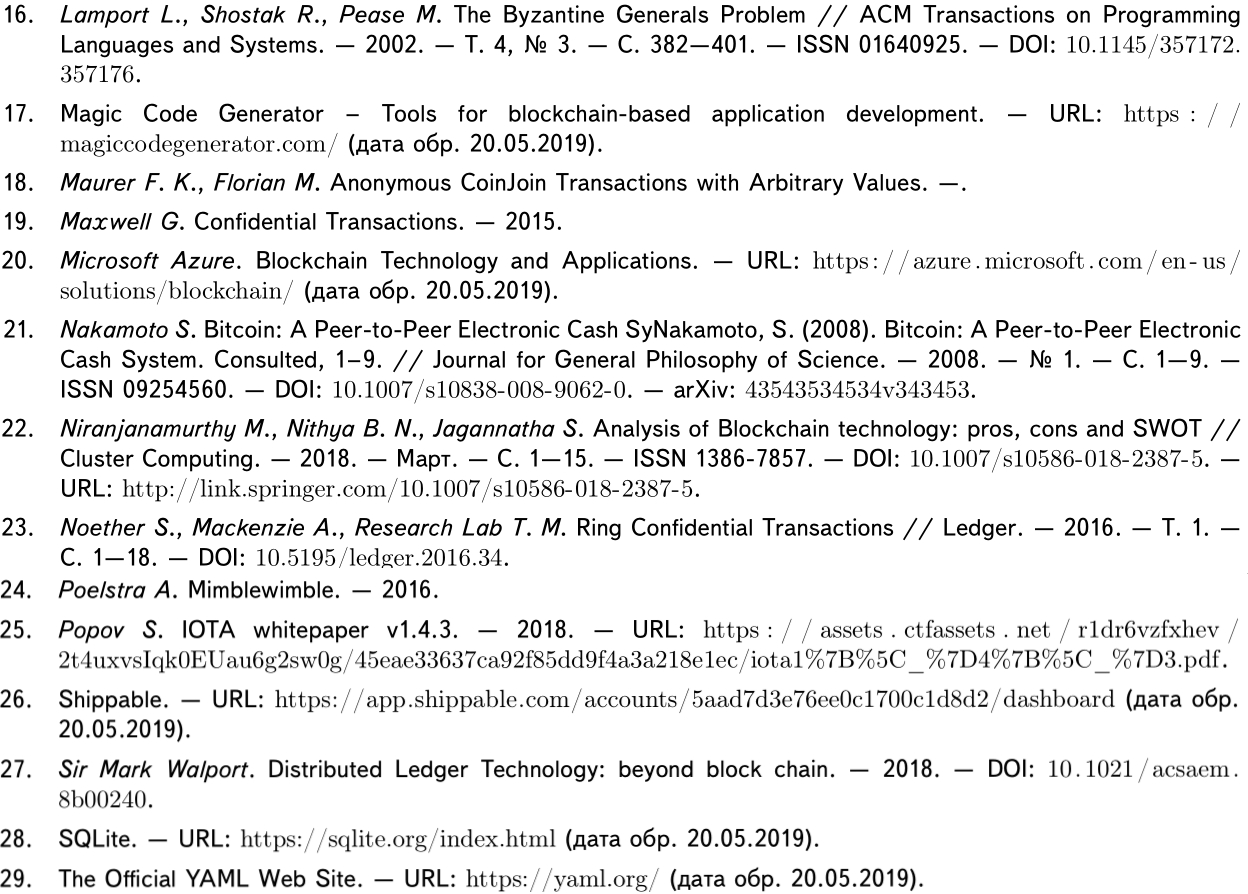
\includegraphics[width=0.85\textwidth]{lib2}
    \end{figure}
\end{frame}

\begin{frame}
    \frametitle{Список используемых источников}
    \begin{figure}
        \centering
        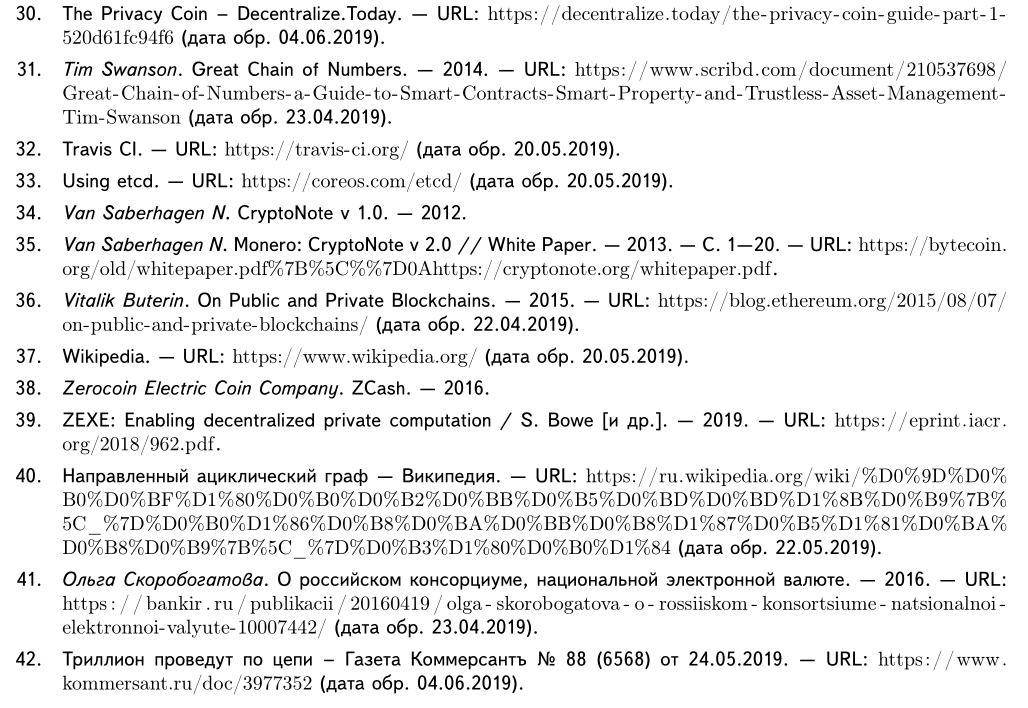
\includegraphics[width=0.9\textwidth]{lib3}
    \end{figure}
\end{frame}

\begin{frame}[c]
\begin{center}
\frametitle{\LARGE Спасибо за внимание!}

{\LARGE \inserttitle}

\bigskip

{\insertauthor}

\bigskip\bigskip

{\scriptsize \color{HSEblue}
    +7-910-008-3926\\
    \href{mailto:kikupriyanov@edu.hse.ru}{kikupriyanov@edu.hse.ru}\\
    \href{mailto:kupriyanovkirill@gmail.com}{kupriyanovkirill@gmail.com}\\
    \href{https://t.me/SsinopsysS}{@SsinopsysS}}

\bigskip\bigskip

{\large \insertdate}
\end{center}
\end{frame}

\begin{frame}
    \frametitle{Процесс работы компоновщика}
    \begin{figure}
        \centering
        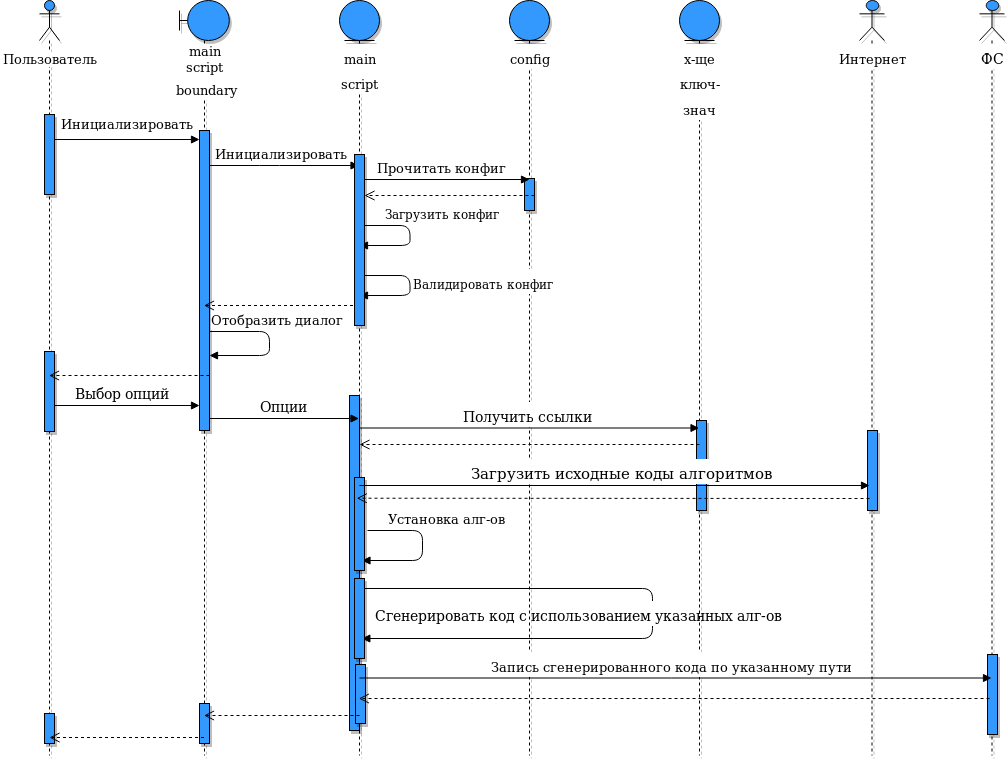
\includegraphics[width=0.8\textwidth]{sequence}
        \caption{\small Диаграмма последовательности работы компоновщика}
    \end{figure}
\end{frame}

\begin{frame}
    \frametitle{Схема хранилища}
    \begin{figure}
        \centering
        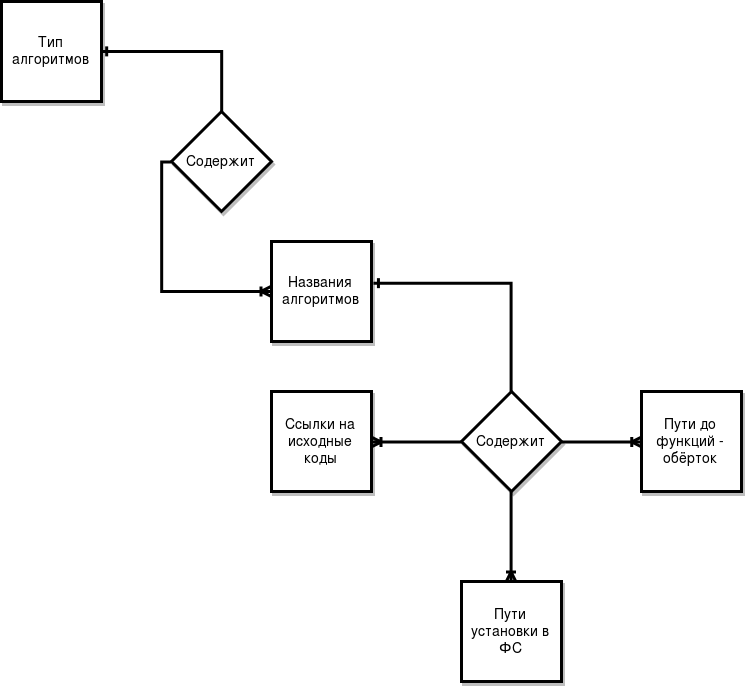
\includegraphics[width=0.67\textwidth]{db}
        \caption{Схема хранилища}
    \end{figure}
\end{frame}

\end{document}


% EOF

